\documentclass{llncs}
\usepackage{epsfig}
\usepackage{graphicx}

\newtheorem{mydef}{Def.}
\newtheorem{myhyp}{Hypothesis}

\usepackage{url}
\usepackage{hyperref}
\usepackage{cleveref}

%\pagestyle{empty}
\pagestyle{headings} 

% ====================================================================

% TODO:
% - clearly point out novelty of this work
% - contribution compared to earlier work

\begin{document}

% ====================================================================
       
\title{Using Metric Space Indexing for Complete and Efficient Record Linkage}

% ====================================================================

\author{Submitted for double-blind review}

%  Hidden For Blind Review
\iffalse  

\author{{\"O}zg{\"u}r Akg{\"u}n\inst{1} \and Alan Dearle\inst{1} \and\\
Graham Kirby\inst{1} \and Peter Christen\inst{2}}

\institute{School of Computer Science, University of St Andrews,\\
St Andrews, Scotland. Contact: \email{ozgur.akgun@st-andrews.ac.uk}
\and
Research School of Computer Science, The Australian National University,\\
Canberra, Australia. Contact: \email{peter.christen@anu.edu.au}}
      
\fi
% ====================================================================

\maketitle

\begin{abstract}

Record linkage is the process of identifying records that refer to the
same real-world entities, in situations where entity identifiers are
unavailable. Records are linked on the basis of similarity between
common attributes, with every pair of records being classified as a
link or non-link depending on the degree of similarity between them.
Record linkage is usually performed in a three-step process: first
groups of similar candidate records are identified using indexing; 
pairs within the same group are then compared in more detail, and
finally classified.
%
Even state-of-the-art indexing techniques, such as Locality Sensitive
Hashing, have potential drawbacks. They may fail to group together some
true matching records with high similarity. Conversely, they may group
records with low similarity, leading to high computational overhead.
%
We propose using metric space indexing to perform \emph{complete} record
linkage, which results in a parameterless record linkage process
combining indexing, comparison and classification into a single step
delivering complete and efficient record linkage.

\end{abstract}

\keywords Entity resolution; data matching; similarity search;
         blocking.

% ====================================================================

\section{Introduction}
\label{sec-intro}

Record linkage, also known as entity resolution, data matching and
duplicate detection~\cite{Chr12}, is the process of identifying and
matching records that refer to the same real-world entities within or
across datasets. The entities to be linked are often people (such as
patients in hospital or customers in business datasets), but record
linkage can also be applied to link consumer products or bibliographic
records~\cite{Chr12}. Record linkage is commonly challenged by the lack
of unique entity identifiers (keys) in the datasets to be linked, which
prevents the use of a database join. Instead, the linkage of records
requires the comparison of the common attributes (or fields) that are
available within the datasets. For datasets that contain information
about individuals, these attributes include the names, address, dates of
birth, and so on, of individuals.

To overcome data quality issues such as typographical errors and
variations (which are common in name and address values~\cite{Chr12}),
approximate string comparison functions (such as edit distance, the
Jaro-Winkler comparator, or Jaccard similarity~\cite{Chr12}) are used to
compare pairs of records, leading to a vector of similarities (one
similarity per attribute/field compared) for each pair. These similarity
vectors are then used to classify the compared record pairs into links
(where it is assumed both records in a pair correspond to the same
real-world entity) and non-links (where the records are assumed to
correspond to two different entities). Various classification methods
have been employed in record linkage~\cite{Chr12,Don15}, ranging from
simple threshold-based to sophisticated clustering, supervised
classification techniques, and active learning approaches~\cite{Wan15}.

Besides the issues of a lack of unique entity identifiers, and data
quality (which will affect linkage quality), record linkage is also
challenged by the increasing sizes of the datasets to be
linked~\cite{Don15}. To avoid full pair-wise comparison of all possible
record pairs (quadratic in the sizes of the datasets to be linked),
blocking techniques, commonly known as \emph{indexing}~\cite{Chr12b},
are used. These split the datasets into smaller blocks in a
computationally efficient way, such that records that are likely to
correspond to the same entity are grouped into the same block. Only
records within the same block are then compared in more detail.

While indexing techniques facilitate efficient linkage of very large
datasets~\cite{Don15}, they generally achieve scalability at the cost
of reduced linkage quality, because potentially true matching record
pairs are removed in the indexing step, leading to a reduction in recall
of the final linkage result~\cite{Chr12}. A variety of indexing
techniques, discussed in more detail in the following section, have
been proposed, ranging from simple phonetic based blocking~\cite{Chr12}
and sorting of the datasets~\cite{Dra12} to locality sensitive hashing
based techniques~\cite{Kim10,Steorts2014}. Techniques for
unsupervised~\cite{Kej13,Ram15} and supervised~\cite{Bil06,Mic06}
learning of optimal blocking schemes have also been proposed.

\begin{figure}[!t]
  \centering
  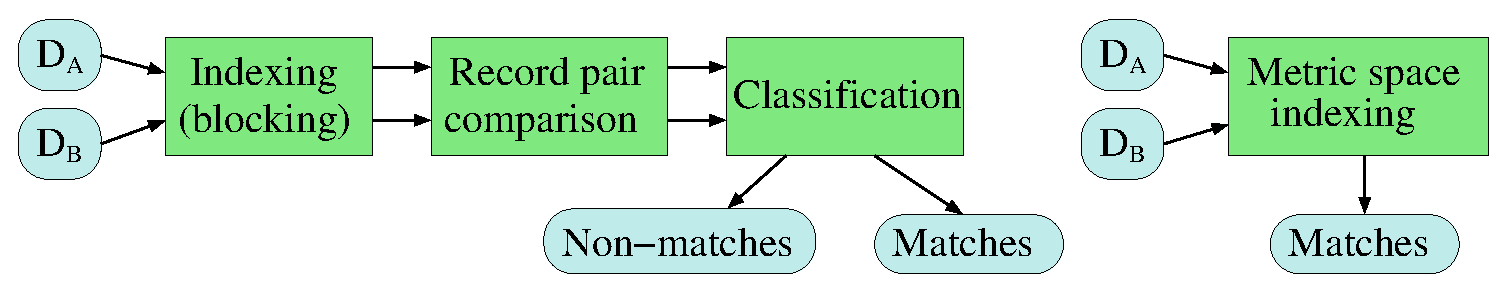
\includegraphics[width=1.0\textwidth]{figures/linkage-process}
  \caption{Overview of the steps of the traditional record linkage
           process (left-hand side) and our proposed metric space
           indexing based approach (right-hand side), as described in
           Sect.~\ref{sec-intro}, where records from two datasets,
           $\mathbf{D}_A$ and $\mathbf{D}_B$, are being linked.}
           \label{fig-rl-process}
\end{figure}

Systems that perform indexing prior to comparison and classification, as
illustrated in Fig.~\ref{fig-rl-process}, add a further practical
complexity to the process. Indexing, comparison and classification are
often conducted using algorithms and parameters selected based on
technical and domain expertise of the user of the record linkage system,
followed by a manual assessment (auditing) of the linkage
outcomes~\cite{Chr12}. If the quality of the resulting links is not good
enough for a certain application, the linkage process needs to be
repeated with different parameter settings and possibly also alternative
algorithms. This can result in a time-consuming and labor-intensive
iterative process. A major challenge is often the heuristic nature of
indexing, where the choice of a certain indexing technique and its
parameters (including which attributes to use in indexing) will
determine the final outcome of a linkage.

\textbf{TODO: GK rewrite this paragraph. Make the connection between completeness and high recall. Define completenes.}
Here we explore how existing indexing techniques can lead to
low recall, even for record pairs that are highly similar and likely
correspond to true matches. As a result, such techniques can lead
to \emph{incomplete} record linkage results. To address this problem,
\emph{metric space indexing} (MSI) can be used to guarantee that all
record pairs, up to a certain distance threshold, are considered in the
record linkage results. MSI also avoids the need for costly detailed
comparison of record pairs with low similarities, which may be inserted
into the same block with traditional indexing techniques. It allows
indexing, comparison and classification to be combined into a
single step, as shown in Fig.~\ref{fig-rl-process}, making the overall
record linkage process simpler, more efficient and more effective than
the traditional approach.


\textbf{Contribution:} The primary contribution of this paper is the novel application of MSI to achieve complete and efficient record linkage, without the need for complex parameter tuning.
We evaluate our approach on several data sets from diverse domains and demonstrate its advantages over
existing indexing techniques for record linkage.

% For final paper:
% The motivation for this work is the Digitising Scotland project (Dibben 2012), which is in the process of transcribing and linking all the vital events recorded in Scotland between 1856 and 1977. This data set will, when complete, include around 14 million birth records, 11 million death records and 4 million marriage records. As part of the work, certain data fields (locations, occupations and causes of death) are also being classified to the relevant standard coding schemes.

% --------------------------------------------------------------------

\section{Related Work}
\label{sec-related}

We now briefly review relevant work in the areas of indexing
for record linkage (for recent surveys see~\cite{Chr12b,Pap16}),
and metric space indexing~\cite{Zezula2010}.

Techniques to link records across datasets have been investigated for
over five decades~\cite{Fel69,New59}, with the scalability of linking
being an ongoing challenge as datasets grow in size and complexity.
Traditional blocking~\cite{Chr12b} uses a set of attributes (known as a
\emph{blocking key}) to insert records that share the same value(s) in
their blocking key into the same block. Only records within the same
block are  compared to each other. To overcome variations and
misspellings, the values used in blocking keys can be phonetically
encoded using functions such as Soundex, NYSIIS, or
Double-Metaphone~\cite{Chr12}. These convert a string into a code
according to its pronunciation, assigning the same code to similar
sounding names (such as `Gail' and `Gayle'). Multiple blocking keys may
be used to deal with the problem of missing attribute values.

A different approach to indexing is the sorted neighborhood
method~\cite{Mon96}, where the datasets to be linked are sorted
according to a \emph{sorting key} (usually a concatenation of the values
from several attributes). A sliding window is then moved over the
datasets and only records within the window are compared. Techniques
that adaptively shrink or expand the window size based on the
characteristics of the sorting key values have shown to improve both
linkage efficiency and quality~\cite{Dra12} over other sliding window
approaches.

These blocking techniques are heuristics, commonly requiring domain
knowledge, such as the choice of appropriate blocking or sorting keys.
Poor choices of blocking attributes result in records being inserted
into inappropriate blocks, and thus true matches being missed. As a
result, such techniques can lead to \emph{incomplete} linkage.
Conversely, many of the record pairs compared in a block may turn
out to have low similarity, corresponding to non-matches, resulting in
\emph{inefficient} linkage.

Locality sensitive hashing (LSH), originally proposed to allow efficient
nearest-neighbor search in high-dimensional spaces~\cite{Ind98}, has
been employed in record linkage as an indexing technique where attribute
values are hashed multiple times, and blocks are created from those
records that share some hash values. \emph{HARRA}~\cite{Kim10} is a
record linkage approach based on MinHash~\cite{Broder1997} and LSH which
blocks, compares, and then merges linked records in an iterative
fashion, where merged records are re-hashed to improve overall linkage
quality. ~\cite{Steorts2014} evaluates two LSH variations, concluding
that in order to get good results, LSH methods must be tuned to the
particular datasets being linked. This requires good quality ground
truth data which may be unavailable or expensive to obtain.

Metric space indexing (MSI) techniques provide indexing structures to
support the comparison of records in one set with those in another,
typically also offering similarity search operations. To create an MSI
data structure, it is necessary to define a distance measure between
records, with certain properties including the \emph{triangle
inequality}. Similarity search operations include
\textit{range-search(q,d)}, where all records within a distance $d$ of a
query record $q$ are identified; \textit{nearest-neighbour(q)},
returning the record with smallest distance to $q$; and
\textit{nearest-n(q,n)}, returning the $n$ closest records to $q$.
\cite{Zezula2010} gives an overview of MSI techniques.
Here we choose one metric space indexing structure, the M-tree
\cite{paolociaccia2m}, and investigate its efficacy for record linkage.

The M-tree is a dynamically balanced tree structure. Every node contains
a reference to a record being indexed, a pointer to its parent, the
distance to its parent, and the node's radius. The radius of a node is
the distance from it to its furthest child. For a parent node with
radius \textit{r}, all its children may be visualised as being contained
within a ball of radius \textit{r} from it.

\cite{Li2006} describes a threshold-based linkage method
using R-trees~\cite{Hjaltason1998}. It demonstrates that high quality
may be achieved using Jaccard similarity over selected record fields.
\cite{Ciaccia97indexingmetric} shows that M-trees are
almost always more efficient than R-trees, hence their use in the
experiments described in this paper.

% --------------------------------------------------------------------

\section{Approach}
\label{sec-approach}

We address the following general record linkage problem: for two
datasets $A$ and $B$, we wish to find, for each record in $A$, all the
records in $B$ that match it. We compare several algorithms for record
linkage: traditional blocking, one incomplete similarity search method,
LSH-MinHash, and one complete method, M-tree~\cite{paolociaccia2m}. We
also use a simple brute-force complete technique as a baseline for
comparison, although this can only feasibly be applied to the smallest
of our datasets. All experiments have a number of parameters to
configure the search space and algorithm behaviour, including a
\emph{distance threshold} specifying a maximum distance, equivalent to a
minimum similarity, for two records to be classified as a link (i.e.\
referring to the same entity).

\textbf{Brute-force:}
Two nested loops are used to compare every record in $A$ with every
record in $B$. Each pair is classified as a link if the distance between
the records is less than the threshold. This approach is guaranteed to
identify all links, with complexity $ O(|A| \times |B|) $.

\textbf{Traditional  blocking:}
The additional parameters are the set of blocking keys and the
normalization encodings applied to each field. These are selected as
described in \cite{Chr12b}, exploiting knowledge of the domain and of
the records being linked, and chosen with the intention of giving the
best possible results for the datasets.
%
Each record in $A$ is placed into the appropriate block based on its
blocking key value. The algorithm then iterates over the records in $B$,
and for each one, compares it with each of the records from $A$ in the
block with the same blocking key value.

\textbf{LSH-MinHash:}
The additional parameters are \emph{shingle size} ($l_{ss}$), \emph{band
size} ($l_{bs}$) and \emph{number of bands} ($l_{nb}$). Each record in
$A$ is placed in an \emph{LSH-MinHash} data structure. First, all the
fields of the record are concatenated, and the result \emph{shingled}
into a set of n-grams with $n = l_{ss}$. Next, a set of 
deterministically generated hash functions are applied to
each n-gram in the set
and the smallest result (the MinHash) of each hash application is added
to a signature for the record. The number of hashes used, and thus the
size of the signature, is set to $l_{nb} \times l_{bs}$. Finally, the
signature is split into $l_{nb}$ bands and the values from each band
are hashed again to create a number of keys. The original record is
added to a map associated with each of the keys. 

To perform linkage, the algorithm iterates over the records in $B$. Each
record is hashed using the procedure described above, to obtain a set of
keys. For each of these keys, the key is looked up in the LSH-MinHash
data structure, and the records from $A$ associated with it added to the
result set. Finally, the record from $B$ is compared in turn with each
record in the result set, with the pair being classified as a link or
non-link based on their distance.

\textbf{M-Tree:} The M-tree linkage algorithm has no additional parameters. In a similar manner to the \emph{LSH-MinHash} approach, M-trees are constructed by supplying the implementation with a set of records and a \emph{distance function}. The distance functions used are the same as those used for \emph{Nested-loop} and \emph{LSH-MinHash} experiments. To perform linkage, the data-structure is searched using a \emph{range-search} query which yields all records within distance $d$ of the query object and all the returned records are directly recorded as links.

% --------------------------------------------------------------------

\section{Experiments and Results}
\label{sec-exp}

We now describe the data sets we use in our evaluation, the setup
employed to evaluate our proposed metric indexing approach and
compare it with traditional blocking techniques, and we then present
and discuss our results~\footnote{The raw data, additional figures and the source code required to run these experiments can be downloaded from here. (Link removed for double blind review)}.

% - - - - - - - - - - - - - - - - - - - - - - - - - - - - - - - - - -

% Peter 31 Oct: table style follows LNCS style guide

\begin{table}[t]
\caption{Characteristics of data sets used in the experiments.}
 \label{table-datasets}
  \centering
  \begin{scriptsize}
  %\addtolength{\tabcolsep}{-0.5pt}
  \begin{tabular}{ccccc}
  \hline\noalign{\smallskip}
  Data set~ & ~Records in~& ~Records in~ & ~Number of true~& ~Entities\\
  name(s)  & dataset1  & dataset2  & matching pairs & linked \\
  \noalign{\smallskip} \hline \noalign{\smallskip}
  CORA  & 1,295 & 1295 & 17,184 & publication-publication\\
  NCVR  & ~224,073~ & 224,061 & ~148,036~ & voter-voter\\
  Isle of Skye & 17,612 & 12,284& 2,900 & birth-death\\
  Kilmarnock  & 38,430 & 23,714 & 8,300 & birth-death\\
  \noalign{\smallskip} \hline
  \end{tabular}
  \end{scriptsize}
\end{table}

\smallskip
\textbf{Data Sets:}
%\label{sec-data}
We used four data sets from three domains in our experiments, as
summarized in Table~\ref{table-datasets}. The first is
\emph{CORA}~\footnote{Available from:
\texttt{http://secondstring.sourceforge.net}}, which contains 1,295
records that refer to 112 machine learning publications. 
It is used as a benchmark data set in the literature for assessing linkage algorithms. Ground truth is provided via a unique
\emph{paper\_id} identifier of the form "blum1993". In this experiment linkage is performed over the same set of records.

The second are two randomly selected sub-sets extracted from the North Carolina Voter Registration
database (\emph{NCVR})~\footnote{Available from: \texttt{http://dl.ncsbe.gov/}}, which were collected in April and June
2014. Each of these contains records of voters including their
first names, surnames, and addresses. Ground truth is provided via a
\emph{NCID} identifier which uniquely identifies a voter.

The last two data sets are historical Scottish records of vital
events (birth, marriages and deaths) one registered on the
\emph{Isle of Skye}, a rural district, and the other
records from \emph{Kilmarnock}, an industrial town. These data sets
were provided to us by historical demographers who extensively
curated and linked both data sets~\cite{reid2002,reid2006}. Both data
sets include the  names, gender, addresses of individuals and their
parents. Ground truth was generated by the demographers based on their
extensive domain knowledge.

% - - - - - - - - - - - - - - - - - - - - - - - - - - - - - - - - - - -

\begin{table}[t]
\caption{Parameter settings used for the different data sets used in
   the experiments,with $d$ the distance threshold used, $l_{ss}$, $l_{sb}$ and $l_{nb}$ the LSH
   shingle size, and the size and number of bands, respectively.}
 \label{table-parameters}
  \centering
  \begin{scriptsize}
  %\addtolength{\tabcolsep}{-0.5pt}
  \begin{tabular}{ccccc}
  \hline\noalign{\smallskip}
  Data set~ & $d$ & $l_{ss}$ & $l_{bs}$ & $l_{nb}$ \\
  name(s) & & & &  \\
  \noalign{\smallskip} \hline \noalign{\smallskip}
  CORA & ~$[0,5,10,\ldots,95,100]$~ & ~$2$~ &
    ~$[2,5,10]$~ & ~$[2,5,10]$~  \\
  NCVR  &  \\
  Isle of Skye &  \\
  Kilmarnock  &  \\
  \noalign{\smallskip} \hline
  \end{tabular}
  \end{scriptsize}
\end{table}

% \smallskip
% \textbf{Experimental Setup:}
% %
% We implemented all techniques described in Sect.~\ref{sec-approach}
% using Java (version 1.8.0\_144) and ran an extensive set of experiments on
% a compute server with 24 Intel(R) Xeon(R) processors running at 2.30GHz, 
% 128 GBytes of main memory and running Red Hat 4.8.5-11.

The parameter settings used in our experiments are summarized in
Table~\ref{table-parameters}.

In all of our experiments we use a single distance metric which is the sum of the Levenshtein distances between the set of fields being compared.

discuss measures used. PC, PQ, num comparisons, time? etc.

\subsection{Cora}

In this section, we perform linkage on the Cora data set using all four approaches presented in this paper: brute force, traditional blocking, LSH and M-Tree.
The brute-force approach is used to establish the threshold value that yields the best possible linkage for the Cora dataset. The threshold value is varied between 0 and 250, \Cref{fig-cora-quality} presents the precision, recall, and F-measure values. 
The linkage results have high precision and low recall for low threshold values, and high recall and low precision for high threshold values.
For this data set, the maximum F-measure value is achieved using a threshold value of 70. This value is data dependent; for different datasets the maximum F-measure will correspond to different thresholds. 
In the rest of this section we fix the threshold value to be 70 which maximises the F-measure for this dataset.

\begin{figure}
\begin{verbatim}
Figure 3 will be a table of Comparisons, F1, precision recall and pairs stuff.
12 ROWS ISH
\end{verbatim}
\caption{Linkage Quality using Brute Force linking on the Cora data set\label{fig-cora-quality}}
\end{figure}

\subsubsection{Traditional Blocking}

Traditionally, blocking is a method for choosing candidates for linkage using manually designed criteria.
Thanks to blocking, a distance is only computed between promising pairs of records.
A major disadvantage of traditional blocking is the need for extra engineering effort.
Bespoke blocking strategies need to be designed for a given data set and application domain.
In this section we experiment with using each key field in the Cora data set as a blocking key one by one, followed by a very permissive blocking key which takes the union of all the blocks attained by using individual key fields.

\emph{AL: The above needs more explanation and not the first bit?}

TODO: Explain pairs-quality and pairs-completeness~\Cref{cora-traditional}.

\begin{figure}
\includegraphics[width=\textwidth]{figures/plotFixedThresholdTraditional2_--_Cora_-_TradBlocking_-_70}
\caption{Blocking Quality using traditional blocking on the Cora data set\label{cora-traditional}}
\end{figure}

\Cref{cora-traditional-prf} plots the linkage quality values obtained by running traditional blocking based linkage at a threshold level of 70. Here, we see that high precision values are possible using blocking based linkage, however the recall (and as a result the F-measure) is poor in comparison to brute-force.

\begin{figure}
\includegraphics[width=\textwidth]{figures/plotFixedThresholdTraditional1_--_Cora_-_TradBlocking_-_70}
\caption{Linkage Quality using traditional blocking on the Cora data set\label{cora-traditional-prf}}
\end{figure}

\subsection{LSH}

LSH is a method for performing blocking without the engineering overhead of traditional blocking.
It is parameterised over two integer values: number of bands, and band sizes~\footnote{LSH can also be parameterised over the shingle size, but in this paper we set the shingle size to 2.}.

\subsection{M-Tree}

M-Tree is a complete method that avoids brute-force search.
In addition, it does not require any additional engineering work, it works with any distance metric.

\begin{figure}
\includegraphics[width=\textwidth]{figures/plotBQ_--_Cora_-_Brute_Force}
\caption{Block Quality - Brute Force\label{cora-block-quality-brute}}
\end{figure}

\begin{figure}
\includegraphics[width=\textwidth]{figures/plotBQ_--_Cora_-_MTree}
\caption{Block Quality - M-Tree\label{cora-block-quality-mtree}}
\end{figure}

\subsection{Historical Demography results}
\begin{itemize}
\item Fig X -1 Repeat of figure 2 with precision recall comparisons etc.
\item Fig X - Kilmarnock M tree plot Precision,recall and F
\item Fig X + 1 - Skye M tree plot Precision,recall and F
\item Fig X + 2 - Mtree F measure and a bunch LSH F measures.
\end{itemize}

\subsection{NCVR}


% --------------------------------------------------------------------

\section{Conclusions and Future Work}

\textbf{Contribution:} The primary contribution of this paper is the novel application of MSI to achieve complete and efficient record linkage, without the need for complex parameter tuning.
We evaluate our approach on several data sets from diverse domains and demonstrate its advantages over
existing indexing techniques for record linkage.

% TODO: check that the above claims have been addressed.



\label{sec-concl}

% --------------------------------------------------------------------

\bibliographystyle{splncs03}
\bibliography{paper.bib} 

% ====================================================================

\end{document}

% ====================================================================

OLD STUFF

\section{The Plan}

\vspace{5mm}

Plan in a bulleted list:

\begin{itemize}
\item Design: Traditionally it has two stages. A blocking method needs to be developed separately from a similarity method. With similarity search based record linkage, there is only one method, and that is the similarity method.
\item Efficiency: I am not convinced of this, but Peter thinks there may be efficiency benefits. The reasoning behind this is that with blocking-based methods we would have to calculate some sort of a similarity value first. This value will only be used for blocking, and later a similarity value between candidate pairs will need to be calculated again.
\item Completeness: Similarity search based methods will be complete (with respect to the given similarity method) whereas blocking based methods (including LSH) are likely to be incomplete (there will be high-similarity pairs which are not places in the same block)
\item Data sets
\begin{itemize}
\item Kilmarnock Birth-Death
\item Skye Birth-Death
\item CORA
\item North Carolina Voter Registration DB
\end{itemize}
\item The following is a list of all methods we thought we would have to compare.
\begin{itemize}
\item Similarity search (M-Tree, others?)
\item LSH-blocking
\item Traditional blocking (e.g. Region, Surname) - \textbf{why this? - this was done in the paper: A Comparison of Blocking Methods for Record Linkage}
\item Sorted Neighbourhood blocking - \textbf{why this?}
\end{itemize}
\item Pairs-completeness and pairs-quality (w.r.t high similarity instead of true-link status). I will expand on this a bit more later.
\item Comparison (for blocking based methods)
		Precision/Recall/F1-Measure
\item Which similarity methods are metric?
\item Run time and memory usage comparisons
\item Theorem. Precision might get better or worse with similarity search based methods, but recall should never get worse.
\end{itemize}

Note: The rest of this paper should be regarded as a placeholder for now.

% ====================================================================

\smallskip
\textbf{MIfile:}
The MIFile \cite{amato2014mi} approach is an inexact technique for performing similarity search based on metric spaces. Using  MI\_file,  each record is represented by the ordering of distances from a collection of reference objects.
% Peter: are these reference object also records? 
It is based on the idea that two records close to each other will have similar neighbours and will thus be represented by similar of distances
% Peter: unclear what you mean with: similar of distances
from the chosen reference objects. 
In order to create the indexes, for each value to be added to the
% peter: value -> record ?
data-structure, first the k nearest reference objects (governed by a fixed parameter) are found, each is given a score (drawn from 1,2,3... based on the reference object's position from the value).
% peter: this is unclear .. I think I understand k-NN: for each
% record you find the k nearest reference objects and you enumerate
% them
Next for each score, a  mapping is created in an inverted index mapping
% peter: unclear..? a mapping in an inverted index mapping?
from the value to the score of each reference object and a representation of the data associated with the reference object and the value inserted.
% peter: unclear: what is "the data" associated with the reference
% object.
In order to perform a \textit{nearest-neighbour} lookup, first the k nearest reference objects (bounded by a second fixed parameter).
% peter: this sentence reads incomplete..?
Next the objects closest to these reference objects are extracted from the inverted map by choosing the neighbours with the highest score.
% Peter: sorry, this is unclear as well. "the objects closest" ->
% records closest? And why highest scores..? Is the closest record
% to a reference object given the highest score (not the lowest
% score - i.e. not 1-closest, 2-closest etc)
Much of the search space may be eliminated by  keeping track of the scores that  can contribute to the nearest neighbours.
% peter: so I guess you use the triangular inequality and the reference
% objects to prune the search space.


\cite{Yu2016} surveys the use of string similarity in record linkage.
Algorithms used to compare two records are characterised as being
character-based or token-based. The first category, including approaches
such as Levenshtein~\cite{Levenshtein66}, uses character differences in
the strings being compared. The second, including techniques such as
Jaccard similarity, treats records as sets of tokens, and utilises set
similarity. There are also hybrids of the two approaches.
% Do we need the rest of this paragraph?
\cite{Yu2016} categorises linkage algorithms as being based on filtering,
verification, or thresholds.
% This is missing some context as to what is going on.
Filtering algorithms generate signatures for each record, construct
inverted lists containing records with common signatures, and prune
records with no common signatures.
% Distance of prefix to what? What is the data in this context?
Verification algorithms calculate the exact distances of a prefix of the
data, and use another technique to estimate the edit distance between
records. If the estimated distance is larger than the desired similarity
threshold, the candidate may be discarded.
% This seems a bit throw-away.
% Also, these aren't themselves linkage algorithms are they?
Threshold-based algorithms include M-trees, Trie-Join, Pass-Join and
Partenum.


%the following is a sentence we culled earlier but may be needed.
We will evaluate the performance of LSH based blocking with regard to the three parameters $l_{ss}$, $l_{bs}$ and $l_{nb}$ in
Sect.~\ref{sec-exp}.


\begin{verbatim}
for each record a in A
    for each record b in B
        classify (a,b) as link if distance(a,b) < threshold
\end{verbatim}




% PAKDD 2018: maximum 12 pages
% Abstract max 200 words
% title, abstract: 1/2 page
% introduction: 1 1/2 page (2 pages so far)
% related work: 1 to 1 1/2 pages (3 pages so far)
% method: 4 pages (7 pages so far)
% experiments: 3 (10 pages so far)
% discussion /conclusion: 1 page
% citations 1

% ====================================================================

% Eamonn ICDM'10 tutorial slides
% - clear problem statement in abstract
% - To convince a reviewer, you must think like a reviewer

% Writing the paper:
% - Make a working title
% - Introduce the topic and define (informally at this stage)
%   terminology
% - Motivation: Emphasize why is the topic important
% - Relate to current knowledge: what’s been done
% - Indicate the gap: what need’s to be done?
% - Formally pose research questions
% - Explain any necessary background material.
% - Introduce formal definitions.
% - Introduce your novel algorithm/representation/data structure etc.
% - Describe experimental set-up, explain what the experiments will
%   show
% - Describe the datasets
% - Summarize results with figures/tables
% - Discuss results
% - Explain conflicting results, unexpected findings and discrepancies
%   with other research
% - State limitations of the study
% - State importance of findings
% - Announce directions for further research
% - Acknowledgements
% - References
%
% - Don’t make the reviewer of your paper think!
% - Reviewers make an initial impression on the first page and don’t
%   change 80% of the time
% - A good introduction with a good motivation is half your success
% - By the end of the introduction the reviewer mustknow.
%   - What is the problem?
%   - Why is it interesting and important?
%   - Why is it hard?why do naive approaches fail?
%   - Why hasn't it been solved before?(Or, what's wrong with previous
%     proposed solutions?)
%   - What are the key components of my approach and results?Also
%     include any specific limitations.
%   - A final paragraph or subsection: “Summary of Contributions”.
%     It should list the major contributions in bullet form,
%     mentioning in which sections they can be found. This material
%     doubles as an outline of the rest of the paper, saving space and
%     eliminating redundancy
% - Unjustified Choices (are bad)
% - Optimal: Does not mean `very good'
% - Proved: Does not mean `demonstrated'
% - Significant: There is a danger of confusing the informal statement
%   and the statistical claim
% - Use all the Space Available
% - Avoid Weak Language: aim, attempt, might, etc.
% - Use the Active Voice
% - ALWAYS put some variance estimate on performance measures (do
%   everything 10 times and give me the variance of whatever you are
%   reporting)

% Figures:
% - Don't cover the data with the labels!
% - Color helps -Direct labeling helps -Meaningful captions help
%
% Common problem with figures:
% 1.Too many patterns on bars
% 2.Use of both different symbols and different lines
% 3.Too many shades of gray on bars
% 4.Lines too thin (or thick)
% 5.Use of three-dimensional bars for only two variables
% 6.Lettering too small and font difficult to read
% 7.Symbols too small or difficult to distinguish
% 8.Redundant title printed on graph
% 9.Use of gray symbols or lines
% 10.Key outside the graph
% 11.Unnecessary numbers in the axis
% 12.Multiple colors map to the same shade of gray
% 13.Unnecessary shading in background
% 14.Using bitmap graphics (instead of vector graphics)
% 15.General carelessness

